%%%%%%%%%%%%%%%%%%%%%%%%%%%%%%%%%%%%%%%%%%%%%%%%%%%%%%%%%%%%%%%%%%%%%%%%%%%%%%%%%%%%%%
%% Author:      Maximilian Stiefel
%% Date:        06.03.2017
%% University:  Uppsala Universitet
%% Department:  Institutionen för informationsteknologi 
%% Course:      Microcontroller Programming
%% Project:     Swakeup
%%%%%%%%%%%%%%%%%%%%%%%%%%%%%%%%%%%%%%%%%%%%%%%%%%%%%%%%%%%%%%%%%%%%%%%%%%%%%%%%%%%%%%

\documentclass{report}

%%%%%%%%%%%%%%%%%%%%%%%%%%%%%%%%%%%%%%%%%%%%%%%%%%%%%%%%%%%%%%%%%%%%%%%%%%%%%%%%%%%%%%
% Preamble
%%%%%%%%%%%%%%%%%%%%%%%%%%%%%%%%%%%%%%%%%%%%%%%%%%%%%%%%%%%%%%%%%%%%%%%%%%%%%%%%%%%%%%

% Encoding of the input
\usepackage[utf8x]{inputenc}
% Geometry stuff
\usepackage[head=24pt,a4paper,lmargin={2.5cm},rmargin={2.5cm},tmargin={2.5cm},
bmargin={2.5cm}]{geometry}
% For graphics
\usepackage{graphicx}
% For code highlighting
\usepackage{minted}
% For shaded
\usepackage{xcolor}
\usepackage{framed}
\definecolor{shadecolor}{gray}{0.9}

% For math
\usepackage{amssymb}

\setlength{\parindent}{0em} 

% For title formatting 
\usepackage{titlesec} 

\titleformat%
{\chapter}%
[block]%
{\bfseries\Huge}%
{\thechapter\hspace{1cm}}%
{0pt}%
{\bfseries\Huge}%

% For SI units.
\usepackage{siunitx}

% Input definition macros
%%%%%%%%%%%%%%%%%%%%%%%%%%%%%%%%%%%%%%%%%%%%%%%%%%%%%%%%%%%%%%%%%%%%%%%%%%%%%%%%%%%%%%
%% Author:	Maximilian Stiefel
%% Date:	06.03.2017
%% University: 	Uppsala Universitet
%% Department: 	Institutionen för informationsteknologi 
%% Course:	Microcontroller Programming
%% Project:	Swakeup
%%%%%%%%%%%%%%%%%%%%%%%%%%%%%%%%%%%%%%%%%%%%%%%%%%%%%%%%%%%%%%%%%%%%%%%%%%%%%%%%%%%%%%

\newcommand{\mytitle}{Swakeup}
\newcommand{\mytypeofwork}{Project Report}
\newcommand{\mycourse}{Microcontroller Programming} 
\newcommand{\myuniversity}{Uppsala Universitet}
\newcommand{\mydepartement}{Information Technology}
\newcommand{\myauthora}{Elmar van Rijnswou (elmarvanrijnswou@hotmail.com)}
\newcommand{\myauthorb}{Maximilian Stiefel (stiefel.maximilian@online.de)}
\newcommand{\myauthorc}{}
\newcommand{\myduedate}{2017-03-10 24:00}
\newcommand{\mytutor}{Uwe Zimmermann (uwe.zimmermann@angstrom.uu.se)}
\newcommand{\mykeywords}{}
\newcommand{\myperiod}{December 2016 - March 2017}


\usepackage{hyperref}
\hypersetup{
	plainpages=false,
	unicode=false,
	pdftoolbar=true,
	pdfmenubar=true,
	pdffitwindow=false,
	pdfstartview={FitH},
	pdftitle={\mytitle},
	pdfauthor={\myauthora ,\space\myauthorb ,\space\myauthorc},
	pdfsubject={\mytypeofwork\space\myduedate},
	pdfcreator={\myauthora ,\space\myauthorb ,\space\myauthorc},
	pdfproducer={\myauthora ,\space\myauthorb ,\space\myauthorc},
	pdfkeywords={\mykeywords},
	pdfnewwindow=true,
	pdfborder={0 0 0},
	colorlinks=false,
	linkcolor=black,
	citecolor=black,
	filecolor=black,
	urlcolor=cyan
}	

\newcommand{\newpar}{\vspace{1em}\\}

\usepackage{amsmath}

\begin{document}

%%%%%%%%%%%%%%%%%%%%%%%%%%%%%%%%%%%%%%%%%%%%%%%%%%%%%%%%%%%%%%%%%%%%%%%%%%%%%%%%%%%%%%
% Ttilepage
%%%%%%%%%%%%%%%%%%%%%%%%%%%%%%%%%%%%%%%%%%%%%%%%%%%%%%%%%%%%%%%%%%%%%%%%%%%%%%%%%%%%%%
%%%%%%%%%%%%%%%%%%%%%%%%%%%%%%%%%%%%%%%%%%%%%%%%%%%%%%%%%%%%%%%%%%%%%%%%%%%%%%%%%%%%%%
%% Author:      Maximilian Stiefel
%% Date:        06.03.2017
%% University:  Uppsala Universitet
%% Department:  Institutionen för informationsteknologi 
%% Course:      Microcontroller Programming
%% Project:     Swakeup
%%%%%%%%%%%%%%%%%%%%%%%%%%%%%%%%%%%%%%%%%%%%%%%%%%%%%%%%%%%%%%%%%%%%%%%%%%%%%%%%%%%%%%

\begin{titlepage}
% temporary margins only for titlepage
\newgeometry{lmargin={2cm},rmargin={2cm},tmargin={1cm},bmargin={2cm}}

%---------------------- Figures --------------------------------------------------

\begin{figure}
	\raggedright
	%\raggedleft
	
\includegraphics[width=0.2\textwidth]{./fig/uppsla_university.png}
\end{figure}

%---------------------- Text -----------------------------------------------------

\begin{center}
	\vspace*{0pt}
	\begin{Huge}
		\textbf{\mytitle}\\
	\end{Huge}
	\vspace*{4em}
	\begin{LARGE}
		\textbf{\MakeUppercase{\mytypeofwork}}\\
	\end{LARGE}	
	\vspace*{2em}
	within the lecture of\\
	\mycourse\\
	\vspace*{2em}
	at \myuniversity\\
	in the Departement of \mydepartement\\
	\vspace*{2em}
	\myauthora{} and \myauthorb{}
	\vspace*{2em}
	Deadline: \myduedate\\
	\vspace*{3em}
	\vfill
%---------------------- Table ----------------------------------------------------
	
	\setlength{\tabcolsep}{24pt}	% change space between rows
	\begin{tabular}{ll}
		Processing Period:&  \myperiod\\
		%&April - Juni 2016\\
		%Matrikelnummern:&4167768\\
		%&1231235\\
		%&4564567\\
		Supervisor:&\mytutor\\
	\end{tabular}
	\setlength{\tabcolsep}{6pt}		% back to default
	\restoregeometry
\end{center}
\end{titlepage}
\clearpage



%%%%%%%%%%%%%%%%%%%%%%%%%%%%%%%%%%%%%%%%%%%%%%%%%%%%%%%%%%%%%%%%%%%%%%%%%%%%%%%%%%%%%%
% Introduction
%%%%%%%%%%%%%%%%%%%%%%%%%%%%%%%%%%%%%%%%%%%%%%%%%%%%%%%%%%%%%%%%%%%%%%%%%%%%%%%%%%%%%%
\chapter{Introduction}
\label{chap:intro}
\section{Idea}
\label{sec:idea}
\section{Sytem Overview}
\label{sec:system}
\begin{figure}[H]
	\centering
	\label{fig:block}
	\includegraphics[width=0.6\textwidth]{../block/block.png}
	\caption{Blockdiagram of the Swakeup wakeup light.}
\end{figure}

%%%%%%%%%%%%%%%%%%%%%%%%%%%%%%%%%%%%%%%%%%%%%%%%%%%%%%%%%%%%%%%%%%%%%%%%%%%%%%%%%%%%%%
% Hardware
%%%%%%%%%%%%%%%%%%%%%%%%%%%%%%%%%%%%%%%%%%%%%%%%%%%%%%%%%%%%%%%%%%%%%%%%%%%%%%%%%%%%%%
\chapter{Hardware}
\label{chap:hardware}
\section{Logic Board}
\label{sec:logic}
The logic board has been realized with the commercial CAD program Altium. The whole circuit fits on one sheet, as the logic board is not a complex design consisting out of very few IC's and passives. 
\subsection{Design choices}
To facilitate all the functionality, certain IC's had to be chosen. The design requirements were to also have a debug option and a way to flash firmware without the need of a specialized programmer. That is why a USB-Serial bridge IC had to be found. There are nowadays quite a few different bridges on the market which all have the same basic functionality that is needed, namely: writing and receiving over a serial port. In order to keep the workload low so that the goal could be reached, an a-synchronous chip was sufficient. Therefor the CP2102 had been chosen. Other competitors with the same functionality were more expensive because they also offered extras that are not needed.\newpar
For \textit{IEEE 802.11} connection the ESP8266 has been chosen. This because it's the cheapest solution on the market, while also providing enough flash and performance to execute the tasks on the module itself, rather than needing a strong microcontroller with it. The ESP8266 itself is preprogrammed with a subset of the Hayes commands. But the firmware can be altered and software can be written in many different languages such as LUA, C++, Python.\newpar
In order to give the user feedback about the time, some interface is needed. As the weather and social media status should be visible this interface has to be a graphic screen of some sorts. Standard LCD's have the disadvantage that they have backlight, which causes annoyances during night when its on. As it acts as a large light source. And if the backlight is turned off, the user won't be able to read out the time. That is why an OLED screen has been chosen, based on the SEPS525F driver. OLED has the advantage that every pixel is lit individually, thus not creating a large light source when only time is displayed. Another advantage is the power consumption, which depends on the state of the screen. Fewer pixels being lit means a lower power consumption. \newpar
Only two microcontroller models were available to choose, as the course required to make use of an 8-bit AVR chip. Either the Atmega, or the more recent XMega. The Xmega has an updated design, and provides more efficient power management due to lower power supply while maintaining performance. Other advantages are a multi level interrupts and more advanced GPIO access. In order to facilitate possibilities to flash the ESP8266 module from the xmega, a large flash size is needed. The xmega with the smallest footprint and largest flash was chosen, which is the xmega128a4u.
\subsection{Implementation}
The XMega will be programmed trough a PDI port. Furthermore four ADC and PWM pins are exposed for use with the power board. The screen is connected via a flat flex connector, rather than soldered directly on the board. This allows for reuse of the screen on further revisions without having to purchase new screens.\newpar
An external crystal is used for the real time clock. This gives the possibility to use the 32 bit real time counter on the XMega which is more precise than using a build in oscillator. Two low side n-channel MOSFETS are connected for reverse voltage protection. \newpar
The full schematics can be found in Appendix \ref{append:logic}.
\section{Power Board}
\label{sec:power}
The whole board design has been made in \textit{KiCAD}. \textit{Git} was used for version control. In the schematics (Appendix \ref{append:power}) one can see that the whole board consists of three main building blocks: Connectors, a LED driver with feedback and two step-down converters. A part of the LED driver is also "abused" to drive the OLED. 
\subsection{Microcontroller Power Supply}
There are two step-down converter ICs on the power board. It is the LM2840 which in combination with a simple voltage divider ensures the 2.8 V for Vcc. All step-down converters use the same inductor with a value of 33 uH. It is a low-cost, quite small, shielded inductor which is ment to be used for switching power supplies. Moreover all step-down converters are enhanced with a SMD schottky diode and a of course SMD capacitor for smoothing the output signal. As it is good practice to do so all ICs are making use of decoupling capacitors. 
\subsection{Designated USB Charging Port}
For charging ones phone the TS30012, another step-down converter IC, is used. The feedback voltage divider of this IC is already onboard and does not need to be provided externally as the IC provides fixed 5 V. The output is connected to a USB connector type A. This IC can deliver up to 2 A. An interesting feature of the phone charging circuitry on the power board is the "Dedicated Charging Port" (DCP) functionality. The TPS2514 is a small, easy-to-use, 6-pin component, which complies to the USB standard and a majority of the minefield of propriatary standards to signal a DCP. What does that mean? Well this means, that if you connect your IPhone, it will know, that it can draw more than 100 mA, which are the minimum provided by a normal USB port. Otherwise the current drawn by the phone will be limited. The charging functionality can be turned on and off via a GPIO pin. The TS30012 comes in a QFN16 package (pad pitch of 0.5 mm) to save space.   
\subsection{HW Debugging}
For testing purposes a lot of test points have been created on the board. Futhermore there are  LEDs for different voltages.
\subsection{RGB LED Driver}
The LED driver consists of an actual power electronics part and a feedback part. The idea is, that the voltage driven through the three color channels of the RGB LED can be controlled by software (PID controller). In the power electronics part there are three analog circuits mainly consisting out of a p-channel MOSFET, which is switched by a NPN bipolar transistor. This bipolar transistor gets its intput signal from the µProcessor (PWM). By pulling the 20 V to GND the PMOS "sees" a negative Vgs and opens.             


%%%%%%%%%%%%%%%%%%%%%%%%%%%%%%%%%%%%%%%%%%%%%%%%%%%%%%%%%%%%%%%%%%%%%%%%%%%%%%%%%%%%%%
% Software
%%%%%%%%%%%%%%%%%%%%%%%%%%%%%%%%%%%%%%%%%%%%%%%%%%%%%%%%%%%%%%%%%%%%%%%%%%%%%%%%%%%%%%
\chapter{Software}
\label{chap:software}
\section{Code Structure}
\label{sec:code_structure}
The code is structured in a layered approach. This has multiple advantages. It's now possible to change microcontroller platform by only having to port the platform layer. Or if a different screen driver is used, only the software driver will have to be ported. Or of the application is meant to be changed, the application layer  has to be adjusted without any changes on the tightly integrated platform code.\\
Other advantages are the reduction of having to test the whole system time after time, as it is possible to rely on the underlying layer if that is tested accordingly.\\
\begin{figure}[H]
	\centering
	\label{fig:code_structure}
	\includegraphics[width=0.6\textwidth]{../block/code_structure.png}
	\caption{The layered approach}
\end{figure}
In fig. \ref{fig:code_structure} the structure is visualized and it can be seen how every layer depends on a lower level layer. Every block can be swapped with different components while the system keeps running, if implemented well without breaches of layering.\newpar
To make this layered code structure a reality, a small operating system has been developed which allows for event driven communication, and a modular approach for driver and sub-systems. This modular approach also makes power saving easier as a module will be uninitialized when it's not used anymore. Removing any possibility for the developer of the system to forget to disable the peripheral/module.\newpar
In fig. \ref{fig:block} the functions of the system can be observed, these functions can be translated into modules and a hierarchy can be created. Along with drivers for the hardware, some software drivers have been written as well. These software drivers provide support for internal development such as logging text in a properly fashion, and creating a way of executing commands on the device. All the platform drivers are interfaces to the system's peripheral. On top of this layer are the actual drivers. This houses the initialization code for the hardware drivers, and gives a way to access the functionality of the hardware without needing to know the registers/commands. The layer above this provides a more generic function set, where no knowledge of the hardware is needed anymore. This can then be used by the last layer, the Application layer. The application layer houses different applications, and a general state of the device can be found inside this layer.
\begin{figure}[H]
	\centering
	\label{fig:block_code}
	\includegraphics[width=0.9\textwidth]{../block/block_code.png}
	\caption{The system structure and hierarchy}
\end{figure}
above in fig. \ref{fig:block_code} this translation from system design to a more refined code structure is shown. A brief description of the required functionality for every block follows. 
\subsection{App layer} The core in the App layer takes care of putting the system in the right state, and decides when to show which application on the screen. Furthermore it establishes the WI-FI connection and requests the data from the Internet that's required for all the other applications. Also it translates commands coming from the UART port into actions. The weather application takes data thats fed from the core, and shows the weather at a given position on the screen. The clock application listens to second pulses and shows the time on the screen, together with an alarm. The time is shown both analogue and digital. The time can be read from the Time module, or be set trough the Core, when it synchronizes with the Internet. The Screen Terminal application redirects all the log output and shows it on the screen. This can be used for debugging. Facebook and mail notifications are shown with the Social application. Finally the Lamp application houses information about different sunsets, and accounts for the right amount of red, green and blue in the light when the alarm goes off.
\subsection{Module layer}
The WI-FI module makes it possible to translate actions as getting the weather and the current time, to udp and tcp requests. The Command module interprets data given from the Terminal and executes a given function paired with the command sent. Everything is written to the terminal via the Log module, which adds extra information to every message, such as the file name, line number and time. The screen module contains functions to draw shapes and images. Time reads the latest known time from the EEPROM after a total power failure, and keeps track of the current time via second pulses. To allow fades in the light, and stable output, a Controller module is available. This reads out the current voltage with which the lamp is being driven, and adjusts the PWM signal accordingly. 
\subsection{Driver layer}
The ESP8266 Driver contains all the communication with the ESP8266 chip and keeps track of the network state. Its also possible to update the firmware of the ESP8266. Terminal is a software driver, with no external hardware dependencies by default. It can, however, use the SEP525F as output for text. The text can be formatted with the Terminal driver. In order to set up the screen and draw pixels, a screen driver is required. The oled screen that is being used, has a SEP525F driver ic. For this a driver has been written.
\subsection{Platform layer}
Every required peripheral has a platform driver. The UART driver has an input and output buffer, and is being used with interrupts. Two UART channels are being used, one for the ESP8266 and one for the USB-Serial converter. The SEP525F has a SPI interface without a need or possibility to read, the SPI driver contains only blocking write. This should be changed to DMA and interrupt transfers. The EEPROM allows to save some settings and time and date on the clock. The timer sets up the real time counter for the second pulses, and has functions to set the PWM of every channel for the power board. And as last, the ADC peripheral. This scales the voltage read from the input pins and provides it to whomever needs the ADC values.
\section{Operating System}
\label{sec:os}
To make the previously discussed layering possible with communication, a small operating system has been developed with a minimum subset of functions. This subset is divided in two parts, Events and Modules.
\subsection{Module}
The modular system is realized by a struct. Every module contains a name, a usage counter, initialize and deinitialize functions, and dependencies. A module can be initialized by the "module\_init" function. This function will check for all the dependencies, whether they are already initialized. If this is not the case, it will be initialized including all the dependencies of the dependency. The "module\_init" function will also call the initialize function, which can be used for a module to set up registers for example. Once a module is not needed anymore, it can be deinitialized with the "module\_deinit" function. This function will decrease the usage counter for every dependency, and once a dependency is not used anymore it will also be deinitialized. This function also calls the deinitialize function of the given module.

\begin{minted}[baselinestretch=1, fontsize=\small, linenos,frame=single,framesep=5pt]{C}
#define MODULE_DEFINE(VAR, DESC, INIT, DEINIT, ...)     \
	Module VAR = {                          	\
		.init = INIT,                           \
		.deinit = DEINIT,                       \
		.cnt = 0,                               \
		.name = DESC,                           \
		.deps = { __VA_ARGS__ }                 \
	} 
MODULE_DEFINE(CORE, "Central core", init, deinit, &TIME, &COMMAND, &ESP8266);
\end{minted}
In the code above a simplified usage example can be seen of this modular system

\subsection{Event}
For communication between modules an event based system has been realized. The developed system does not have any kind of priority for events, and events can be ignored if the event buffer is full because of a too heavy event. Every event contains a counter for debugging purposes, a pointer to data that can be given along with the event, and a description. An event can be created by use of the following code:
\begin{minted}[baselinestretch=1, fontsize=\small, linenos,frame=single,framesep=5pt]{C}
#define EVENT_REGISTER(eventName, desc)\
	Event eventName = \
	{.eventId = __COUNTER__, .data = 0, .description = desc, .descLen = sizeof(desc) }
EVENT_REGISTER(EVENT_UART_DELIMITER, "Got UART delimiter");
\end{minted}
Events alone do not serve any purpose without listeners. Thus it's possible to register listeners in the event system. With the "event\_addListener" function a module can listen to a certain event and provide a function to be called upon the reception of such an event. This can be seen in the code below:
\begin{minted}[baselinestretch=1, fontsize=\small, linenos,frame=single,framesep=5pt]{C}
event_addListener(&EVENT_UART_DELIMITER, callback);
\end{minted}
The listeners can be removed with the "event\_removeListener" function. The adding listeners is usually done in the initialization function, as the modules require these events during the period that they are active. In order to fire an event to all the listeners the following example can be used: 
\begin{minted}[baselinestretch=1, fontsize=\small, linenos,frame=single,framesep=5pt]{C}
event_fire(&EVENT_UART_DELIMITER, SYSTEM_ADDRESS_CAST (&delimiters[USART_ID][i]));
\end{minted}
This line of code will fire a EVENT\_UART\_DELIMITER event, and adds some information to go with it.\newpar
In order for these events to be processed the "event\_process" has to be called. This should be the only function called in the infinite while loop of the system. A way to save energy is to pass functions to the event system if the system is capable of a sleeping functionality. Now the system will sleep whenever there are no more events to process, or wake up when an interrupt occurs.

\section{Realization}
\label{sec:realization}
The function of this chapter is to get a deeper understanding of the modules and code that has been written. Due to time constraints and hardware failure, the following modules were not realized: "Lamp, Social, Wi-Fi, Controller, ADC, EEPROM". Thus these modules will not be discussed in this chapter. 
\subsection{Platform}
Starting with the most tightly with the microcontroller integrated layer.
\subsubsection{UART}
The UART module delivers all the communication to the USB-Serial converter and ESP8266. The code has been kept as generic as possible so that adjustments to the external hardware has no influence to the driver code. It would even be possible to move to a different xmega model with more USART ports since a macro is used for generating the interrupt code. Every USART port has a status, an array with delimiters, an in and output buffer, a sending status and an id. The status contains variables for the buffers, and allows for a ring-buffer usage. A ringbuffer is chosen as it has little overhead compared to lists or queues, the order of the data matters, and we don't expect to go outside of our given buffer capacity. The delimiters are used for the USART to listen to certain characters on the receiving data. Once there is a match an event will be fired. The example below shows the usage of this delimiter.
\begin{minted}[baselinestretch=1, fontsize=\small, linenos,frame=single,framesep=5pt]{C}
uint8_t uart_add_delimiter(char delimiter, USART_t * port);
static void callback(Event * event, uint8_t * data) {
	if(event == EVENT_UART_DELIMITER){
	struct UartDelimiter * delimiter = (struct UartDelimiter*)data;
		if (delimiter->port == &ESP_UART_PORT) {
			//Read buffers etc
		}
	}
}
static uint8_t init(void) {
	uart_add_delimiter('\n', &ESP_UART_PORT);
	event_addListener(&EVENT_UART_DELIMITER, callback);
	return 1;
}
\end{minted}
In this example, a certain module will tell the UART module to listen for a new line character, and the module will subscribe to the event. The UART module passes the delimiter information with it, so that there is knowledge about how much data can be read since the last delimiter event.\\ 
The interrupts are generated with the macros that can be found at appendix \ref{append:usartinterruptgen}.
The following code can be used to generate the interrupt code for every USART channel:\newpage
\begin{minted}[baselinestretch=1, breaklines=true, fontsize=\small, linenos=true,frame=single,framesep=5pt]{C}
USARTRXCISR(USARTE0, DEBUG_UART,     USARTE_ID, received);
USARTDREISR(USARTE0, DEBUG_UART,     USARTE_ID);
USARTRXCISR(USARTD1, ESP_UART_PORT,  USARTD_ID, );
USARTDREISR(USARTD1, ESP_UART_PORT,  USARTD_ID);
\end{minted}
Since the system could be writing to the buffer that is being handled in the interrupt, a lock has been implemented to prevent unexpected outcome. One lock waits while the lock signal is freed, while the other lock function returns a 0 upon failure to acquire the lock.
\begin{minted}[baselinestretch=1, fontsize=\small, linenos,frame=single,framesep=5pt]{C}
#define lock(id) while (outBufferLock[id]); outBufferLock[id] = 1
#define unlock(id) outBufferLock[id] = 0

static inline uint8_t softlock(uint8_t id) {
	if (outBufferLock[id]) return 0;
	outBufferLock[id] = 1;
	return 1;
}
\end{minted}
The USART on both channels have the same settings: 8 bit words, medium level interrupts and a baudrate of 115200. This baudrate can go higher once the whole system is tested with good results.
\subsubsection{SPI}
The SPI driver is incomplete as is, a lot of performance optimizations can and should be done. One of the biggest disadvantages at the moment is that it is blocked writing. When a lot of data is being sent consecutively by the SPI driver, the event buffer fills up and might even get full. Interrupt based design should be looked at and investigated, as this would still allow the events to be handled. The caveat with this, however, is that a large buffer has to be allocated for the SPI. And memory is costly. DMA is another technique to solve the problem, this would eliminate the need for a CPU at all and give the system all the time to process the other tasks. One needs to be cautious, as DMA has overhead on low data amounts.
\subsubsection{Timer}
The Timer design is incomplete, and only houses a RTC. Due to a hardware failure, the internal crystal is being used. Which implies a worse accuracy than an external one. However since the most recent time can be retrieved from the internet this is not a major issue. Future additions to the Timer module include: Alarm function for timeouts on waiting, PWM functionality and using the 32 RTC with the external crystal. The Timer module is set up to use it's overflow interrupt. The period is set to 1023. As soon as the counter reaches 1024, a second pulse event will get fired and the run time will get incremented.
\subsection{Driver}
One step up gives the communication with external hardware.
\subsubsection{SEPS525F}
As mentioned before, the screen uses a SEPS525F IC. This driver drives allows for driving screens with a resolution of up to 160x128 pixels with 18 bit combined color. This means that there are 6 bits for blue, 6 bits for green and 6 bits for red. However this would require to send 3 bytes for 2 bits of color precision. There is also a 16 bits combined color option available, which has been used in this driver. 5 bits for blue, 6 bits for green and 5 bits for red. A 24 bit color (8 bits per color, 0-255) can be converted with the following define:
\begin{minted}[baselinestretch=1, fontsize=\small, linenos,frame=single,framesep=5pt]{C}
#define SEPS525F_TO656(r,g,b)((r>>3)<<11)|((g>>2)<<5)|(b>>3)
\end{minted}
The SEPS525F has three data interfaces that could be used: SPI, RGB, Parallel. In retrospect a parallel interface would have given major performance advantages. However due to time constraints a SPI interface has been chosen. The clock frequency of the SPI is set at the CPU speed divided by two. Which is a clock of 8 MHz when not in any power saving mode.\newpar
The SEPS525F has two modes, a data mode and a command mode. With the command mode a register can be set. In order to achieve this the register will be written first, while clearing the RS and the CS pin. Once the register is written, the RS pin will be set while keeping the CS pin low. After the data is written the CS pin will be set.
\begin{minted}[baselinestretch=1, fontsize=\small, linenos,frame=single,framesep=5pt]{C}
static void SEPS525F_reg(int idx, int value) {
	SEPS525F_PORT.OUTCLR = SEPS525F_CSB | SEPS525F_RS;
	spi_write_blocked(idx);
	SEPS525F_PORT.OUTSET = SEPS525F_RS;
	SEPS525F_PORT.OUTCLR = SEPS525F_CSB;
	spi_write_blocked(value);
	SEPS525F_PORT.OUTSET = SEPS525F_CSB;
}
\end{minted}
This can be seen in the code above. The driver gives the possibility to draw a single pixel, but it's significantly faster to write multiple pixels at once. For this a region that will be drawn on has to be set. Then the driver ic will expect a certain amount of pixels, which have to be written as data. According to the datasheet special scrolling features should be available, however this is not explained later on in the datasheet. There are a lot of parameters that can be set for the screen, such as duty cycle, frame rate, driving currents. The explanation of all these can be found in the datasheet, just like the recommended values. The given initialization sequence of the datasheet did not work, so an Arduino library has been ported successfully\cite{github:oled}.
\subsubsection{Terminal}
The Terminal driver gives the possibility to format strings, and outputs the formatted strings to a sink. The default sink writes to the USB-Serial IC via the UART driver. Formatting is done via the tinyprintf library\cite{sparetimelabs:tinyprintf} and implements the 'd' 'u' 'c' 's' 'x' 'X' formats.
\subsubsection{ESP8266}
The ESP8266 is a low cost Wi-Fi module which can be flashed with own firmware. In a next version this own firmware will be developed, however for now the standard firmware is used. UART is used to communicate with the module, via an Hayes command set based protocol\cite{lonestar:at}. The commands implemented allow for basic HTTP get requests. Due to time constraints it was not possible to finalize the usage of the module. Networks can be scanned, and a connection with a wireless action point can be established. But there is no functionality beyond that.
\subsection{Modules}
Although all the drivers talked about before make use of the Module system, they are not located on the Module layer. This is a naming convention mistake.
\subsubsection{Command}
The Command module has the purpose of setting up an accessible possibility to execute commands received by the USB-Serial connection. It is possible to register up to 26 commands. One for every letter in the alphabet. A command can be registered by use of the following code:
\begin{minted}[baselinestretch=1, fontsize=\small, linenos,frame=single,framesep=5pt]{C}
command_hook_description(
	'T', &terminalCommand, "Log sink    T<option> options: U(Uart) S(Screen)\0"
);
\end{minted}
It takes 3 arguments, the first one being the letter the command is tied to. The second one is a function pointer for the callback. And the third one is a usage description that can be requested by the user by writing a '?' to the terminal. In fig. \ref{fig:command_usage} an example output can be seen.
\begin{figure}[H]
	\centering
	\label{fig:command_usage}
	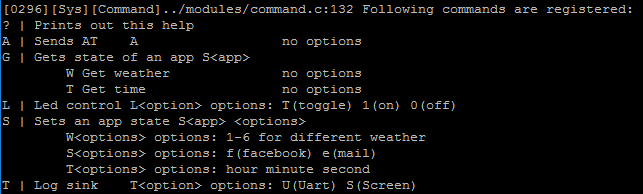
\includegraphics[width=1\textwidth]{./fig/command_usage.png}
	\caption{Response of a question mark}
\end{figure}
It's up to the developer to parse the string that is passed with the command. An example input string could be:"ST 12 23 34" which sets the time to 12:23:34. The callback will receive the same string as thats sent, minus the command character. Some helper functions have been written such as "command\_next\_int" to make parsing easier. Parsing the example string is done in the following code:
\begin{minted}[baselinestretch=1, fontsize=\small, linenos,frame=single,framesep=5pt]{C}
uint8_t index = 1;
if(data[index-1] == 'T'){
	uint32_t hour = command_next_int(&index, data, len);
	uint32_t minute = command_next_int(&index, data, len);
	uint32_t second = command_next_int(&index, data, len);
}
\end{minted}
\subsubsection{LOG}
Almost every driver or module has a dependency on the LOG driver. In order to use the logging functionality, a file first has to initialize the logger. this is done by calling:
\begin{minted}[baselinestretch=1, fontsize=\small, linenos,frame=single,framesep=5pt]{C}
LOG_INIT("Core");
\end{minted}
This is required to keep track of where the logging happens. There are multiple levels of logging, which currently all have the same effect other than the name, except for the "LOG\_ERROR" function. The error log function halts the system. In a future build there should be a possibility to set a general log level so that log statements with less importance than the general log level will not be written. Every log is translated to the following three statements:
\begin{minted}[baselinestretch=1, fontsize=\small, linenos,frame=single,framesep=5pt]{C}
#define LOG_INTERNAL(LEVEL, MSG, ...) \
	log_message("[%04d][%s][%s]%s:%d ",timer_runTime(),LEVEL,log_name,__FILE__,__LINE__);   \
	log_message_p(PSTR(MSG), ##__VA_ARGS__);                                                        \
	log_message("\r\n")
\end{minted}
An example like:
\begin{minted}[baselinestretch=1, fontsize=\small, linenos,frame=single,framesep=5pt]{C}
LOG_SYSTEM("Received command: %c", command);	//command is a character
\end{minted}
Produces the following string on the sink: "[2727][Sys][Command]../modules/command.c:157 Received command: T". The string contains the absolute runtime, what kind of log it was (debug, system, warning), the filename and the file line. The strings are saved in the flash to save memory. If the sink for the terminal changes, so does the output for the logger, as its depending on the terminal. The screen can be used to log to. This can be seen in fig. \ref{fig:screen_logger}.
\begin{figure}[H]
	\centering
	\label{fig:screen_logger}
	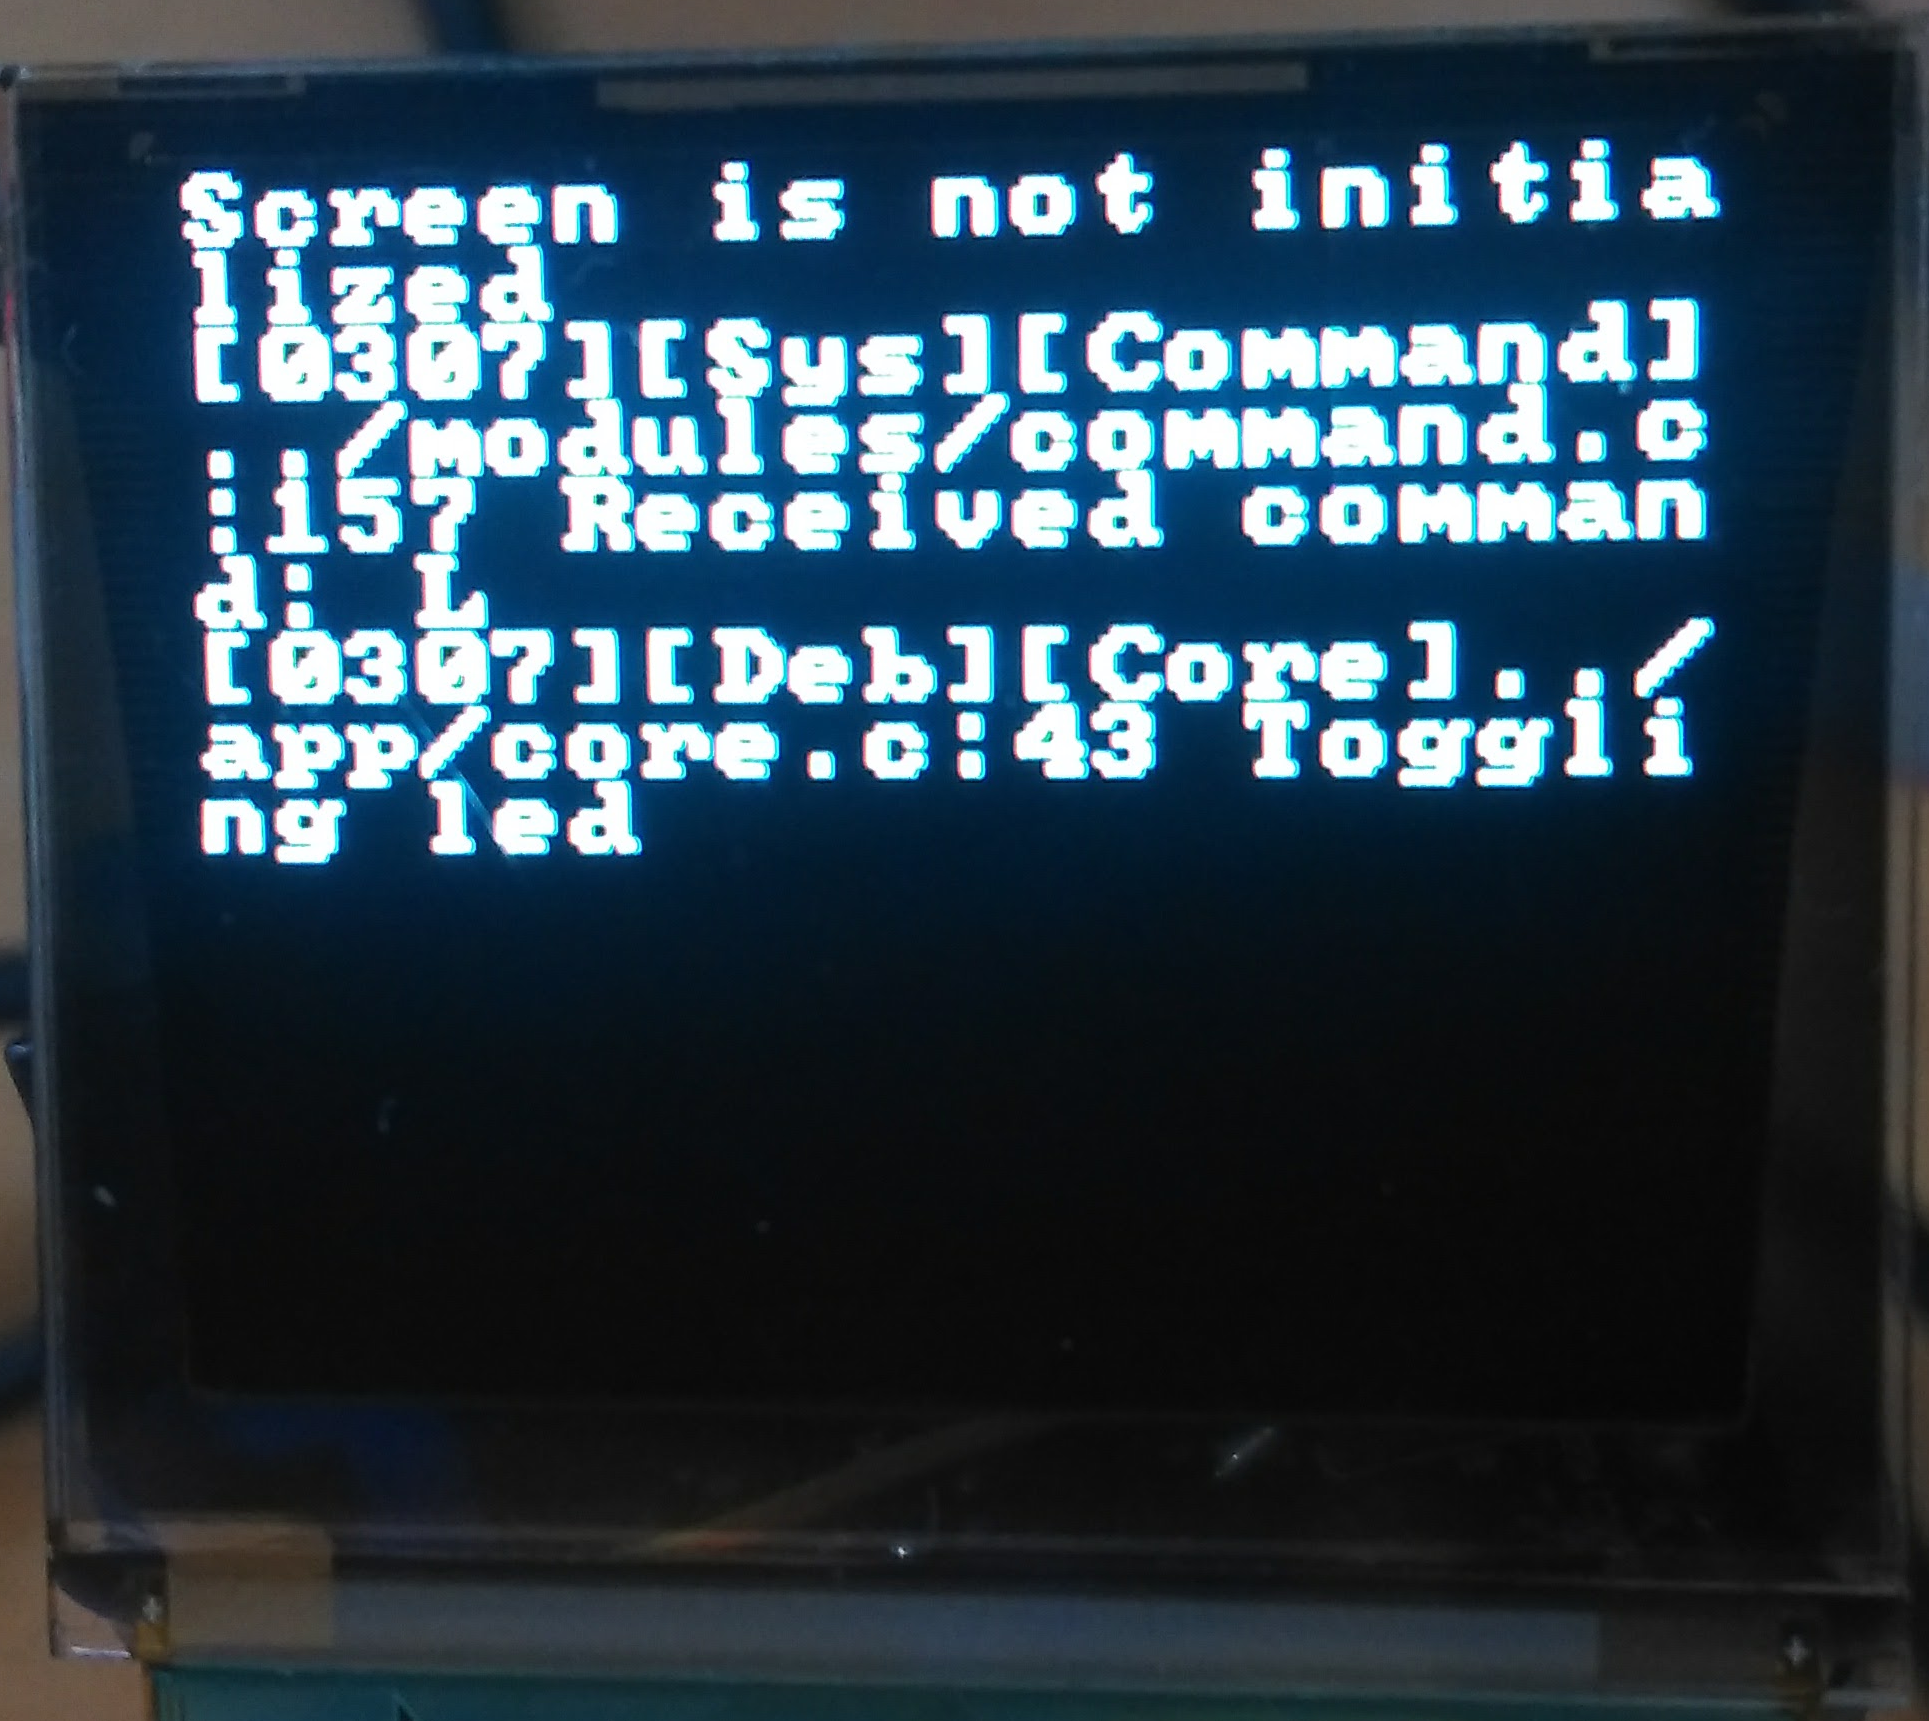
\includegraphics[width=0.4\textwidth]{./fig/screen_logger.png}
	\caption{Redirecting the output to the screen}
\end{figure}
However this has to be used carefully, as writing to screen takes significantly longer than outputting it over UART. So the system might freeze in case of too much text to show.
\subsubsection{Screen}
The Screen module contains routines for drawing shapes, images and text on the screen. Currently implemented shapes include: Rectangle, filled rectangle, circle, filled circle, pixel, and line. These shapes are drawn with the color that is currently set. Images can be drawn both from flash and from memory. Better practice reads them out from flash, as there is little memory available. A start and stop function is available. This can be used to denote whether the shapes should be filled, or whether only the outline should be drawn. Another future addition can speed up the drawing significantly when a data start and data end command will be sent upon calling start and stop. This is not implemented in the current version.
\subsubsection{Time}
The Time keeps track of time offline. It does so by keeping track of hours minutes and seconds, and incrementing them accordingly upon every second pulse generated by the Timer driver. The time can also be set via a function.
\subsection{App}
This layer is the least elaborated, as it has the last priority since it would not work without the layers before it regardless.
\subsubsection{Clock}
The clock application draws a clock, analogue and digital. It gets update every second pulse, and also redraws in that case. The SPI connection is not capable enough to show a smooth analogue clock as is, which causes slight stutters when drawing. This behavior could be resolved when programming even more efficiently, one way of tackling this problem would be to draw the lines first to a buffer, which then is drawn as an image. This would provide a more efficient pipeline for drawing the clock, at the cost of memory. Otherwise a compromise will have to be made, and the analogue clock could be replaced by a large digital one. Or removing the second digit. The positions of the lines are static and calculated beforehand.
\subsubsection{Weather}
The weather application currently does nothing else than draw an image based on a weather condition given. It makes use of one large image consisting multiple tiles for different weather conditions (rain, snow, sun, overcast) which are being drawn via screen routines.
\subsubsection{Core}
The Core translates all the commands given to actions. The debug LED can be toggled, AT commands can be sent, the sink for the terminal can be changed, time and weather can be set. The core also decides where to draw what application. Currently this results in fig. \ref{fig:clock_weather} below.
\begin{figure}[H]
	\centering
	\label{fig:clock_weather}
	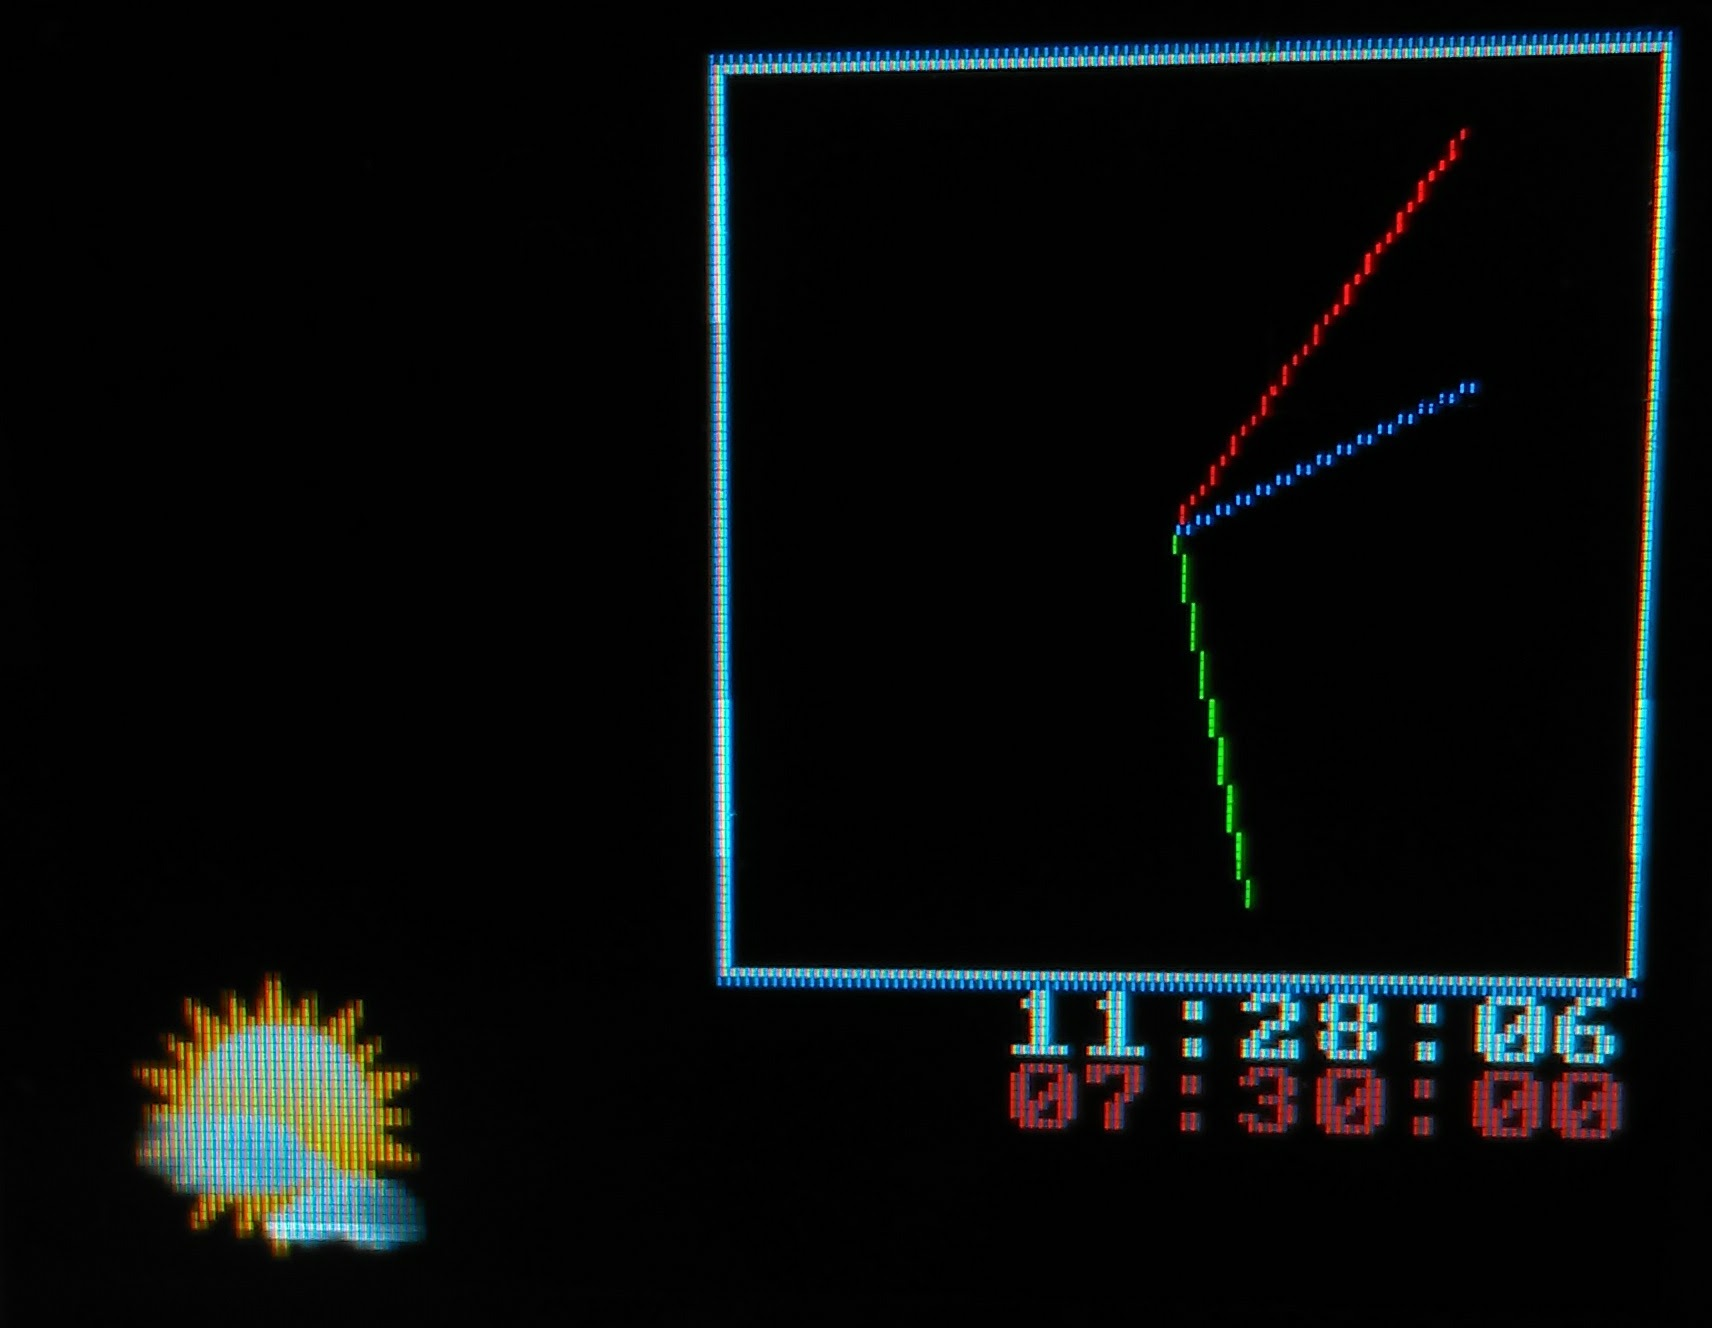
\includegraphics[width=0.4\textwidth]{./fig/clock_weather.png}
	\caption{Displaying the clock and the weather}
\end{figure}

%%%%%%%%%%%%%%%%%%%%%%%%%%%%%%%%%%%%%%%%%%%%%%%%%%%%%%%%%%%%%%%%%%%%%%%%%%%%%%%%%%%%%%
% Satus Quo and Outlook
%%%%%%%%%%%%%%%%%%%%%%%%%%%%%%%%%%%%%%%%%%%%%%%%%%%%%%%%%%%%%%%%%%%%%%%%%%%%%%%%%%%%%%
\chapter{Status Quo and Outlook}
\label{chap:status}
\section{What works? What does not work?}
\label{sec:what}
The hardware right now is in revision 2.0. There has been one revision before the current one. This revision has been fabricated in january 2017 and the design process began in november 2016. There were some mistakes on the first hardware revision, which were not fixable so easily, especially because of the fact, that everything is quite small. Table \ref{tab:hw} gives an overview of the current satus of the hardware.   
\begin{table}[H]
\centering
\begin{tabular}{lll}
\textbf{HW Block}  	& \textbf{Working}& \textbf{Problem}  	\\\hline
USB Charging 	& \checkmark	& 				\\
OLED Driver  	& \checkmark    & 				\\
Vcc for µC   	& \checkmark    & 				\\
IEEE 802.11   	& \checkmark    &                             	\\
USB2UART	& \checkmark	&				\\
LED Driver	&		& Wrong footprint assignment	\\
Crystal		&		& Wrong pin assignment		\\
USB DCP		&		& Further tests necessary	\\
\end{tabular}
\caption{Hardware Overview: What works? What does not?}
\label{tab:hw}
\end{table}
Table \ref{tab:sw} deals with an overview about the status of the software. 
\begin{table}[H]
\centering
\begin{tabular}{lll}
\textbf{SW Block}  	& \textbf{Working}& \textbf{Problem} 	\\\hline
UART 		& \checkmark	& 				\\
SPI	  	& \checkmark    & 				\\
EPROM   	& \checkmark    & 				\\
Timer   	& \checkmark    &                             	\\
ADC		& 		& 				\\
PWM 		&		&				\\
ESP8266		& \checkmark	& 				\\
Terminal	& \checkmark	& 				\\
SEP525F		& \checkmark	& 				\\
Wifi		& 		& 				\\
Command		& \checkmark	& 				\\
Log		& \checkmark	& 				\\
Screen		& \checkmark	& 				\\
Timekeeper	& \checkmark	& 				\\
Controller	&		&				\\
Core		& \checkmark	& 				\\
Weather		& \checkmark	&				\\
Clock		& \checkmark	&				\\
Social		& 		&				\\
\end{tabular}
\caption{Software Overview: What works? What does not?}
\label{tab:sw}
\end{table}

\section{Outlook}
\label{sec:outlook}
Hopefully the LED driver will work with the next revision. The new boards have not arrived until the deadline. As soon as the hardware is working, the controllers will be implemented in software. 
\newpar
Aditional funtionality will be implemented e.g. connecting you calendar to the device and seing your daily agenda when you wake up. Also there is no housing yet.    

\end{document}
